\section{Methodology}
\label{sec:casa}

\subsection{Motivation}
\label{sec:motivation}
% \changnan{!!!! The idea is reasonable, but the content is weak after all. This part requires a more formal discussion, or a practical verification.  !!!
% Check back later.}
% For brevity, we abuse the notation and use $\mathbb{E}_\pi$ to represent either $\mathbb{E}_{s \sim d^\pi} \mathbb{E}_{a \sim \pi(\cdot | s)}$ or $\mathbb{E}_{a \sim \pi(\cdot | s)}$ depending on whether $\mathbb{E}_{s \sim d^\pi}$ is needed.
We use $V_{\theta}$ to estimate $V^\pi$, $Q_{\theta}$ to estimate $Q^\pi$ and $\pi_{\theta}$ to represent the policy,
where $\theta$ represents all parameters to be optimized.
{\colorred In this work, there is one backbone and two individual heads after the backbone. 
The advantage function and the policy share one head, and state value function is the other head. 
Hence the policy reuses all parameters of value functions except that temperature $\tau$ is only for the policy.
We keep $\tau$ static in this work.}
% \haosen{or we should point out here that V and Q or pi share most of parameters but not all. a past reviewer misunderstood this.}
We use \textbf{E} to represent the policy evaluation, which gives the ascent direction of the gradient by $\theta \leftarrow \theta + \eta \mathbb{E}_{\pi} [(Q^{\pi} - Q_{\theta}) \nabla_{\theta} Q_{\theta}]$. 
We use \textbf{I} to represent the policy improvement, which gives
% The policy gradient theorem ~\citep{sutton} shows that $\nabla_\theta \mathcal{J} = \mathbb{E}_\pi [(Q^\pi-V_\theta) \nabla_\theta \log \pi_\theta]$, so the gradient ascent with \textbf{I} is defined as 
$\theta \leftarrow \theta + \eta \mathbb{E}_\pi [(Q^\pi-V_\theta) \nabla_\theta \log \pi_\theta]$.

\begin{figure}[t]
\centering 
\vspace{-0.5cm}
\begin{minipage}[t]{0.38\linewidth}
\centering
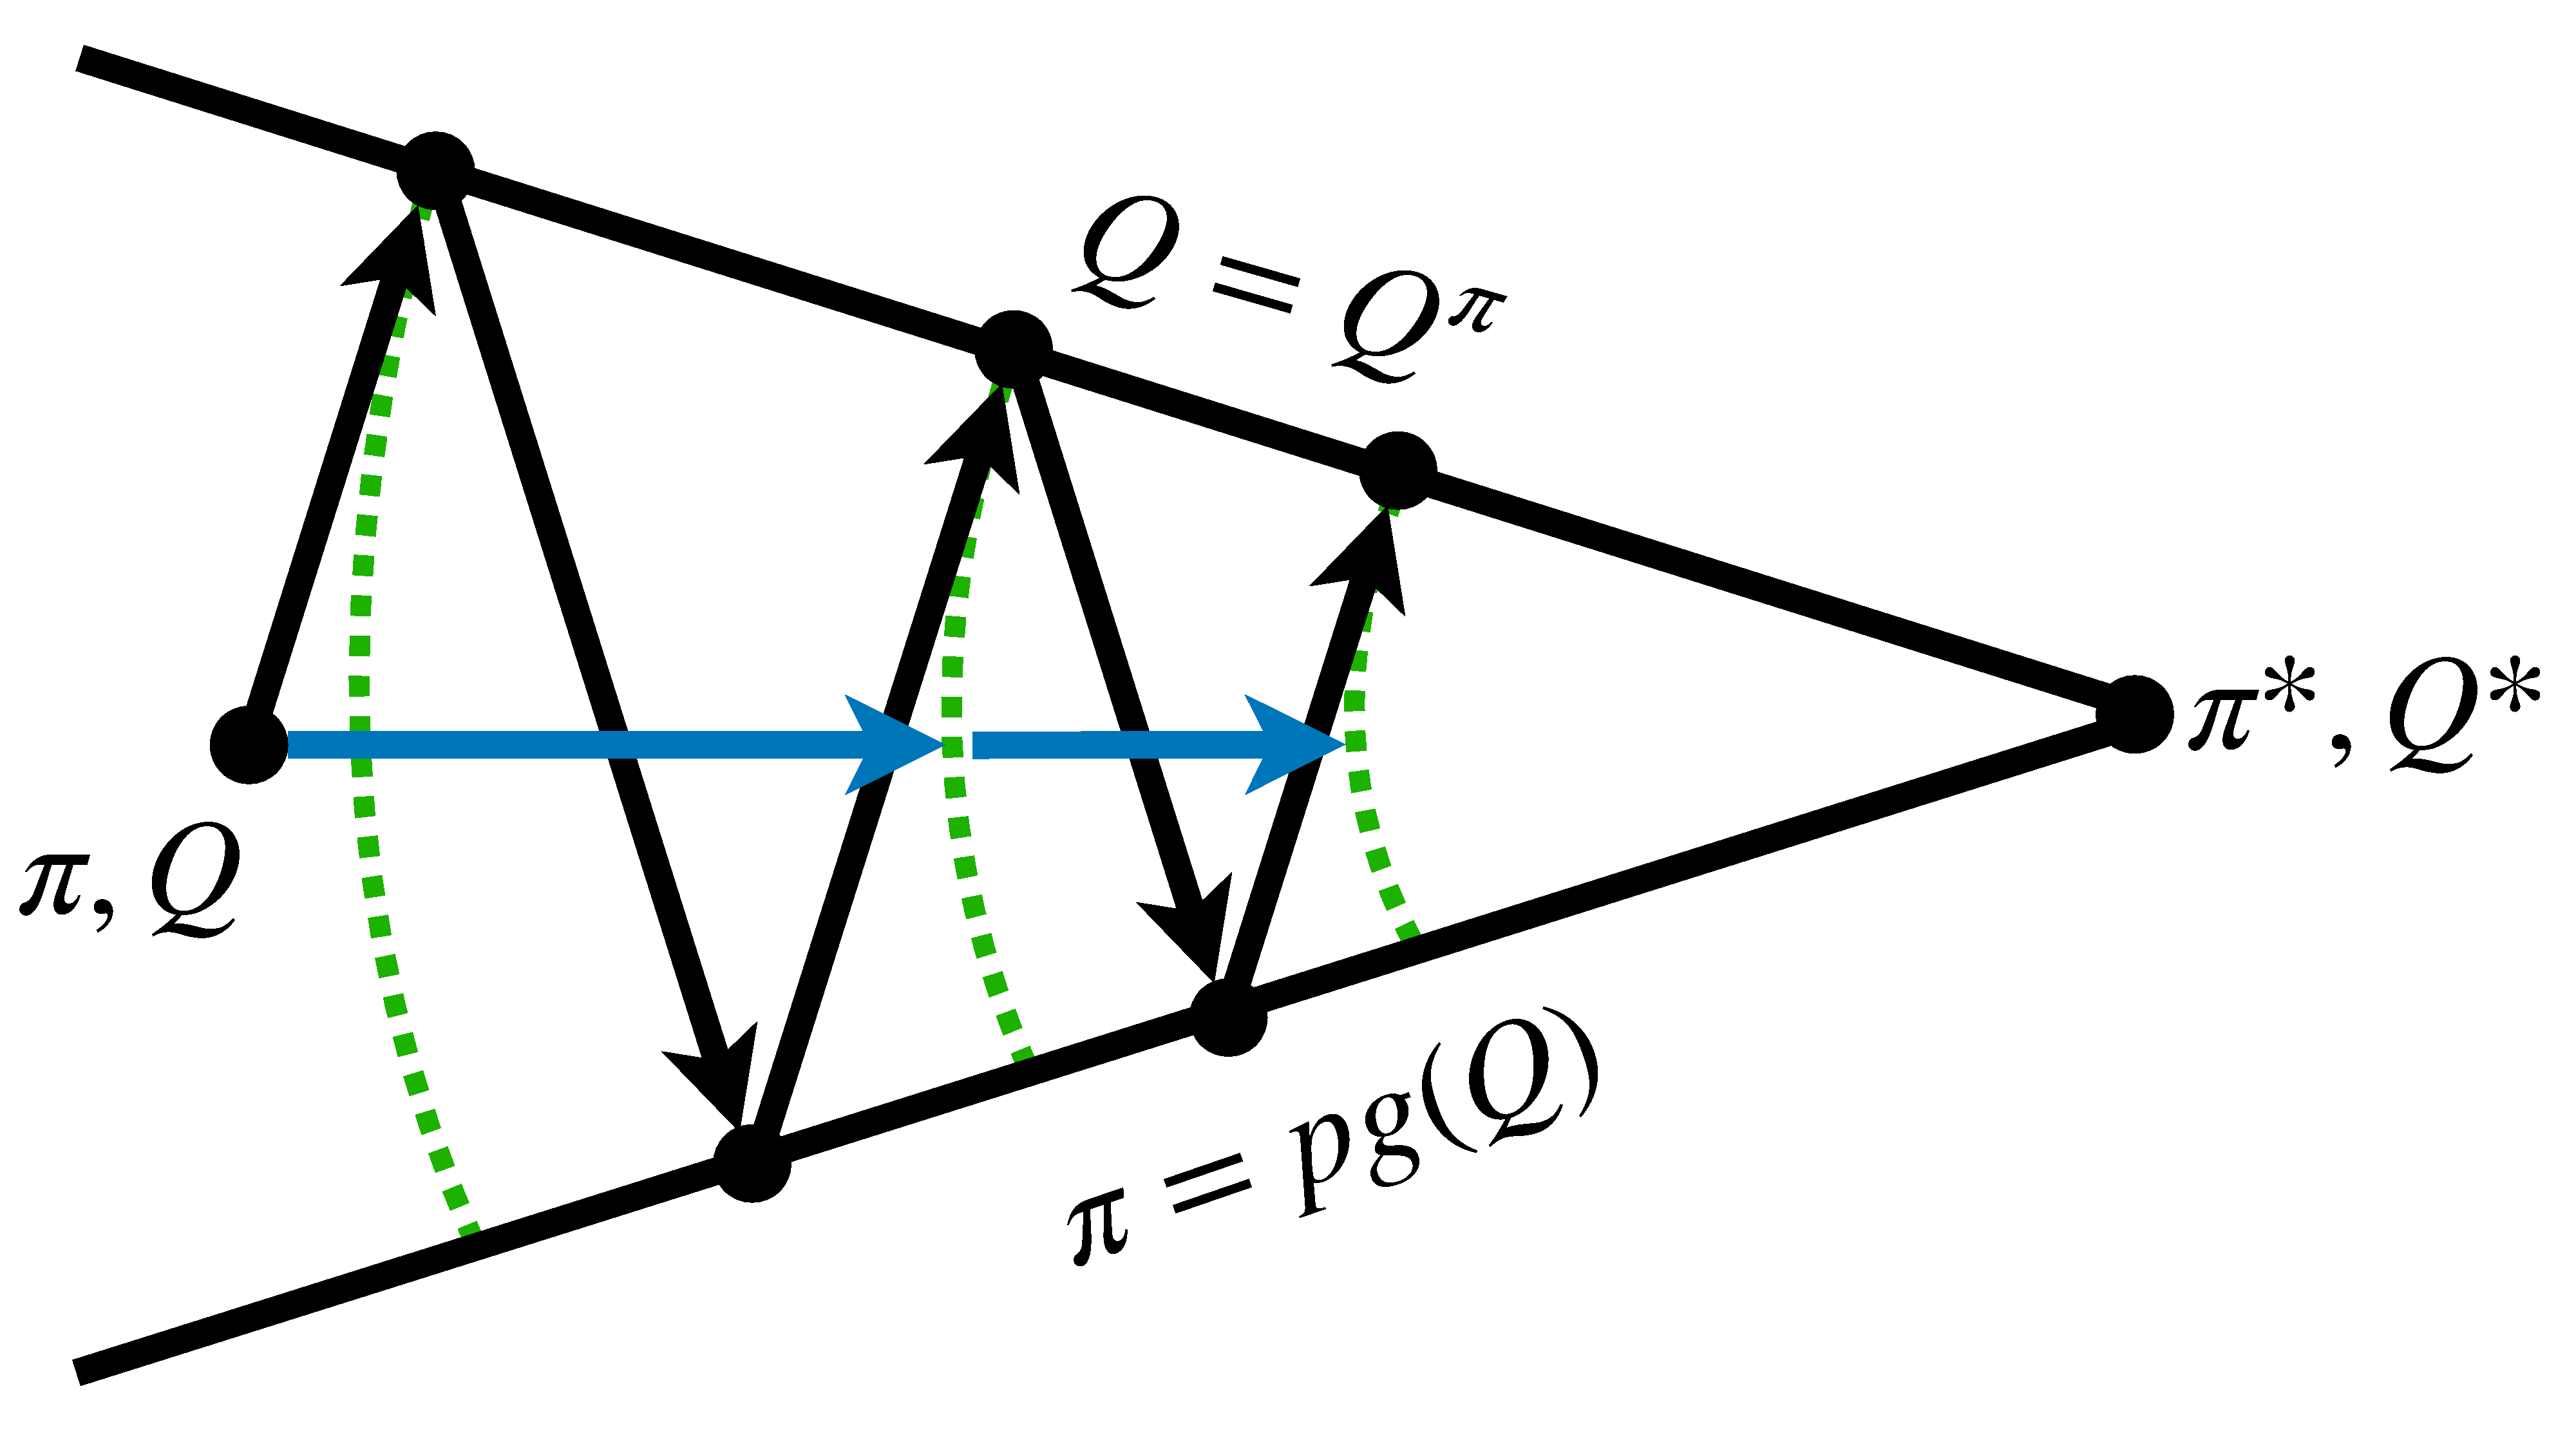
\includegraphics[width=0.95\linewidth]{body/figures/GPI.pdf}
\caption{ \small 
The GPI process in our work. 
Unlike ~\citep{sutton}, we evaluate $\pi$ by $Q$ instead of $V$, and we improve $\pi$ using policy gradient ascent ($pg$ for brevity) instead of greedy. The learning procedure is shown by the black arrows, i.e., $\textbf{E}\rightarrow\textbf{I} \rightarrow \textbf{E} \rightarrow \textbf{I} \cdots$. 
} 
\label{fig:gpi}
\vskip -0.2in
\end{minipage}
\hfill
\begin{minipage}[t]{0.58\linewidth}
\centering
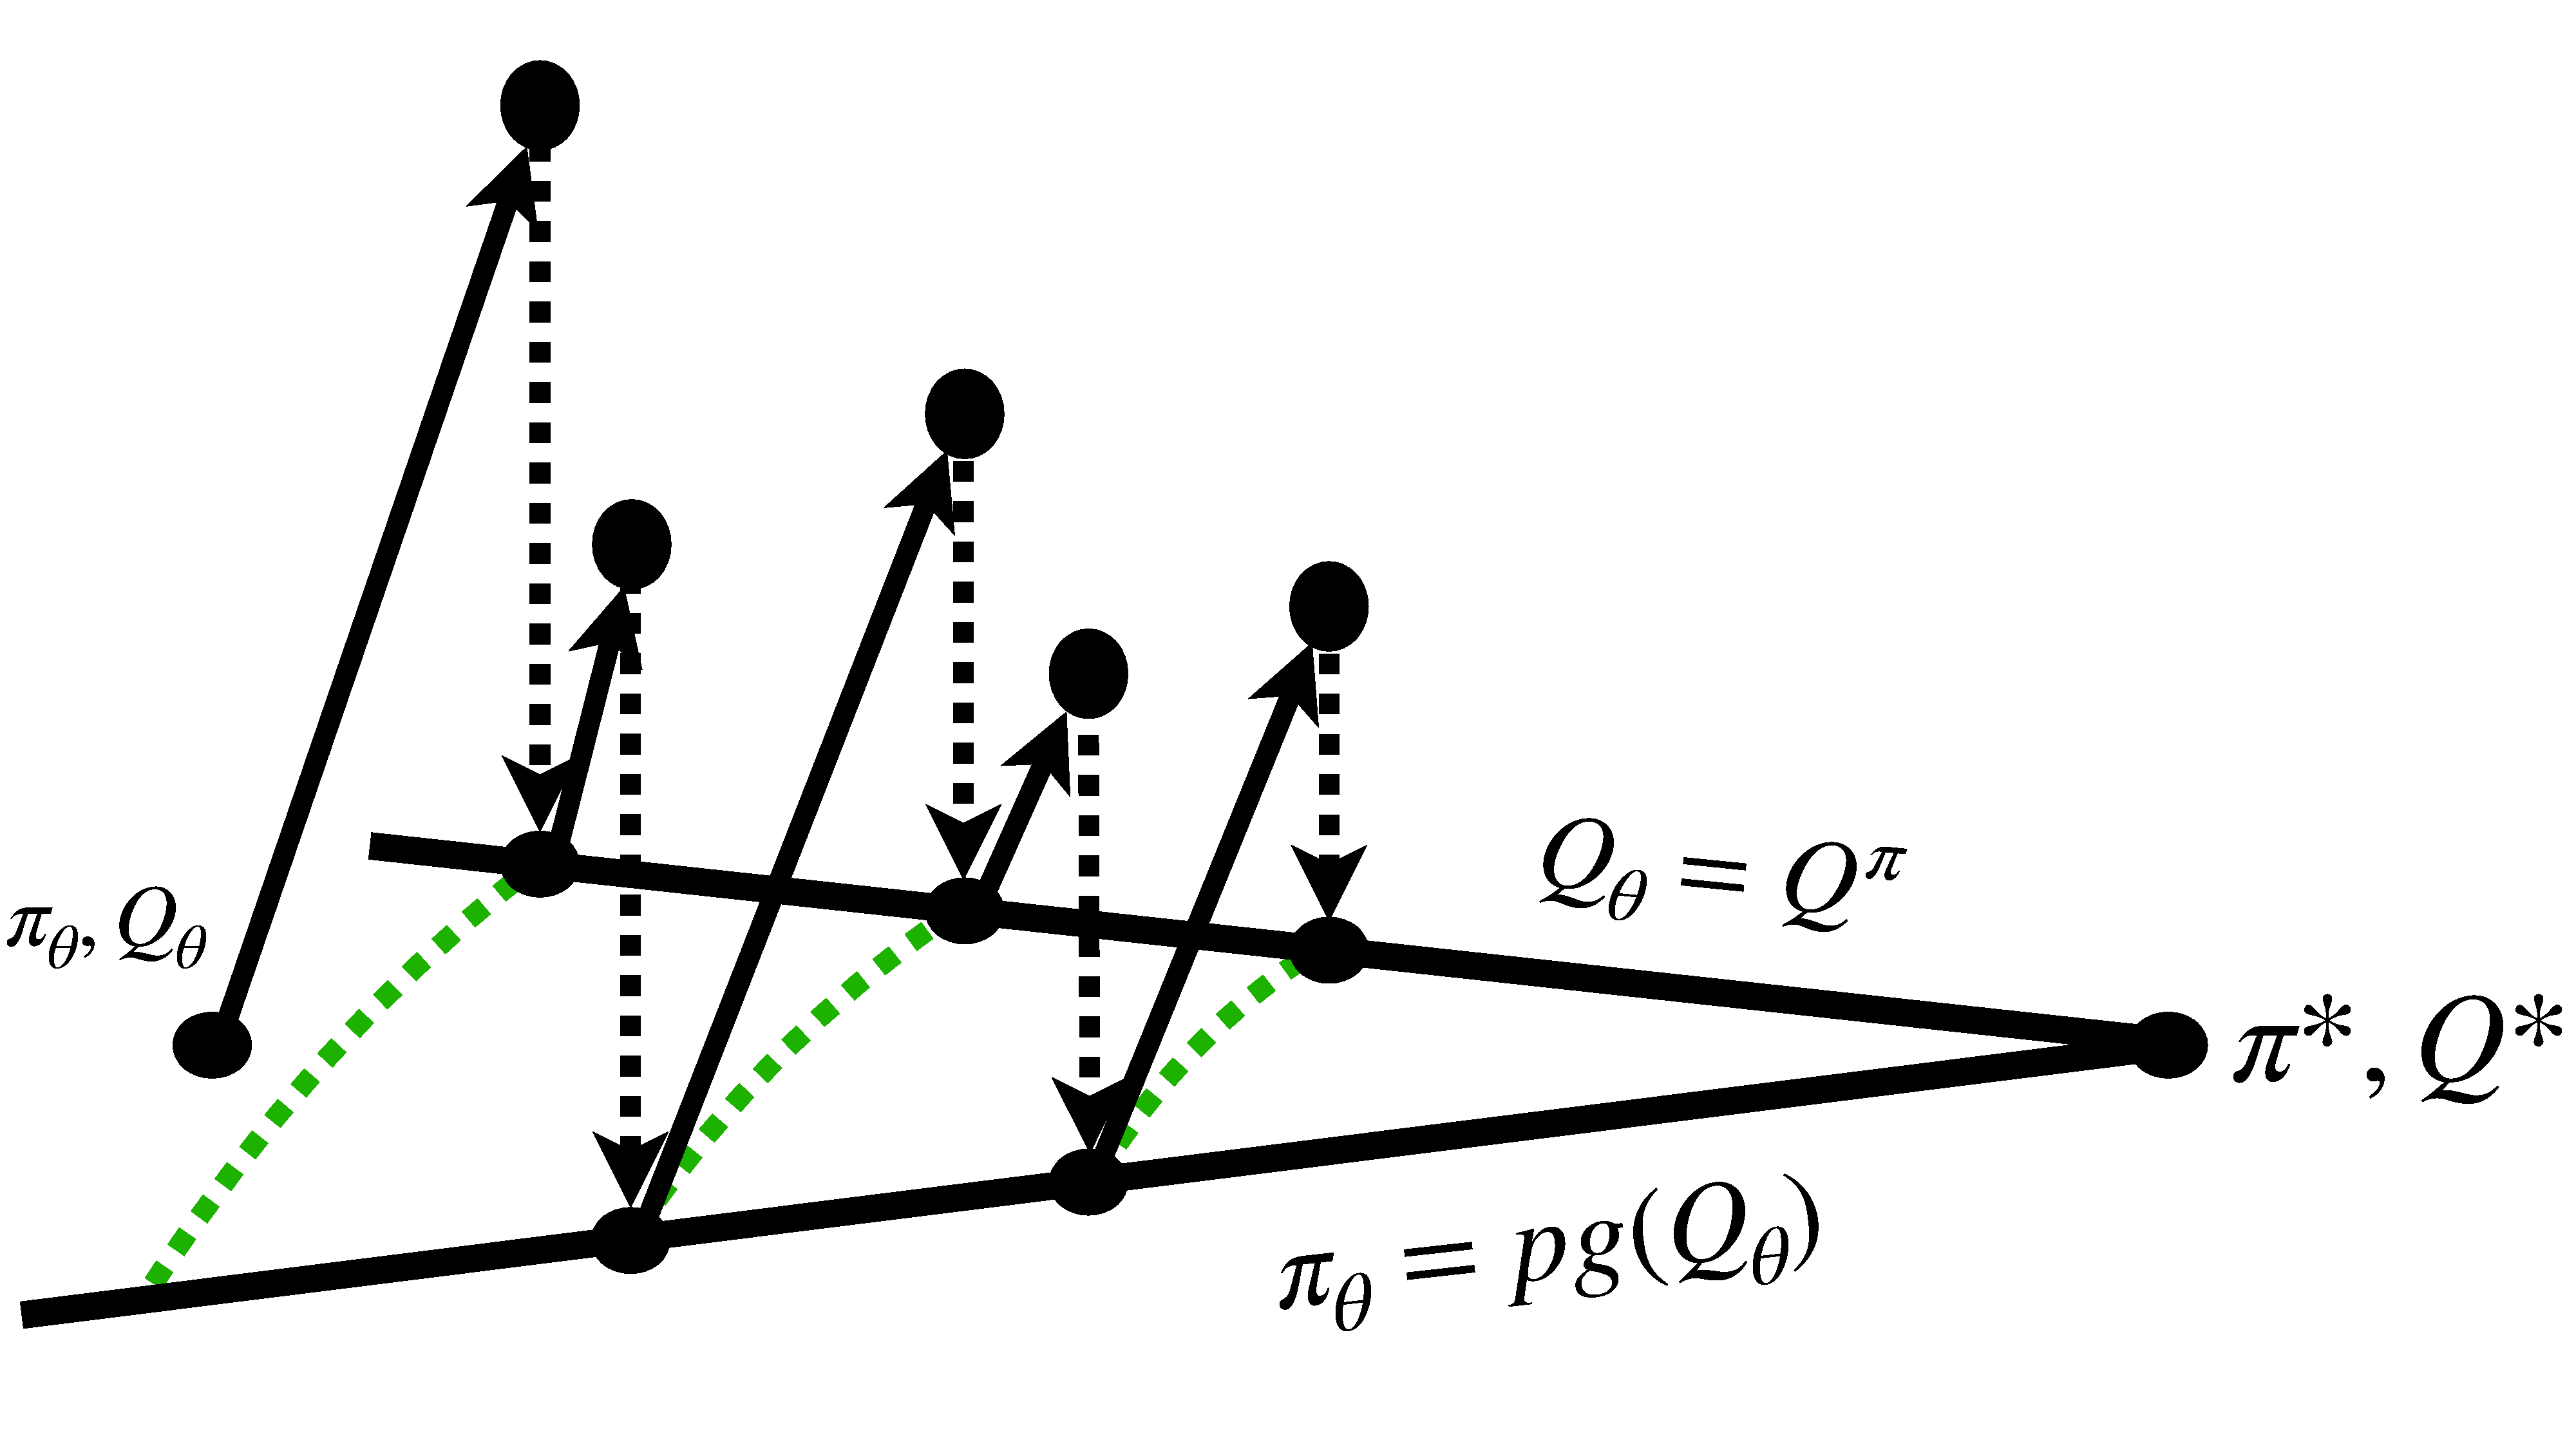
\includegraphics[width=0.65\linewidth]{body/figures/GPI2.pdf}
\caption{\small 
GPI with function approximation. 
% \haiyan{where the ideal policy is desired to select the greedy action with maximum Q value but in reality it's hard to achieve. To minimize the divergence, we project policy and value with operator $p$}.
% \changnan{This description is not accurate. }
Due to the constraint of approximated function space, the ideal policy iteration cannot be actually achieved. The underlying process of GPI with function approximation can be regarded as doing policy improvement and policy evaluation in an ideal space then being projected back into the approximated function space ~\citep{sutton, op_reinforce}.
% The black arrows represent policy improvement and policy evaluation. 
% The dotted arrows represent the projection into the approximated function space.
% The learning process is represented by the black arrows and dotted arrows, $ \textbf{I} \rightarrow \textbf{P}_\textbf{I} \rightarrow \textbf{E} \rightarrow \textbf{P}_\textbf{E} \rightarrow \cdots$.}
%  \haosen{project the ideal objective calculated by equation to a neural network that try to be close to it, see ~\citep{op_reinforce}'s operator D  } 
% \haosen{Here, the projection is a mapping from the ideal function into the neural network support function space.}
 }
\label{fig:gpi2}
\end{minipage}
\vskip -0.1in
\end{figure}

Let's recap the GPI process as shown in Figure \ref{fig:gpi}.
To get rid of the function approximation error, we first assume the approximation function enjoys infinite capacity. 
We use $<x, y>$ to denote the angle between two vectors, where $<x, y> = \arccos (\frac{x\cdot y}{||x||\cdot||y||})$ {\colorred with $\arccos: [-1, 1] \rightarrow [0, \pi]$}. 
We define an important notion $\beta$, which represents the angle between the gradient ascent directions of \textbf{I} and \textbf{E}, as follows,
{\colorred 
\begin{equation}
    \beta \overset{def}{=} <\mathbb{E}_\pi[(Q^\pi-Q_\theta)\nabla_\theta Q_\theta],\, \mathbb{E}_\pi[(Q^\pi-V_\theta) \nabla_\theta \log \pi_\theta]>.
\end{equation}
}
% $\beta \overset{def}{=} <\nabla_\theta Q_\theta,\, \nabla_\theta \log \pi_\theta>$ 
% Since $Q^\pi-Q_\theta$ and $Q^\pi-V_\theta$ are two scalars, when $\nabla_\theta Q_\theta \propto \nabla_\theta \log \pi_\theta$, the two sides of $\beta$ meet.
% As \textbf{I} and \textbf{E} are perpendicular to each side of $\beta$, they become parallel arrows on opposite directions. 
{\colorred When $\beta = 0$ i.e.$\cos(\beta) = 1$, \textbf{I} and \textbf{E} become parallel to each other,  which is the blue arrow in Figure \ref{fig:gpi},
and there is no conflict between the gradient ascent directions of $\textbf{I}$ and $\textbf{E}$ anymore.
When $\beta = \pi / 2$ i.e.$\cos(\beta) = 0$, \textbf{I} and \textbf{E} are perpendicular. 
When $\beta = \pi$ i.e.$\cos(\beta) = -1$, \textbf{I} and \textbf{E} are toward exactly opposite directions. }
% except for the step size that is factored by $Q^\pi-Q_\theta$ and $Q^\pi-V_\theta$. 
% In a special case where $\nabla_\theta Q_\theta \propto \nabla_\theta \log \pi_\theta$ but $Q^\pi-Q_\theta$ and $Q^\pi-V_\theta$ have opposite signs, we have $\beta = \pi$ and we call it $\beta = 0$ since the gradients are still parallel except for their pointing directions.
% For brevity, we denote $\textbf{IE} \overset{def}{=} \textbf{I} \rightarrow \mathbb{E}$.

% \begin{figure}[t]
% \centering
% 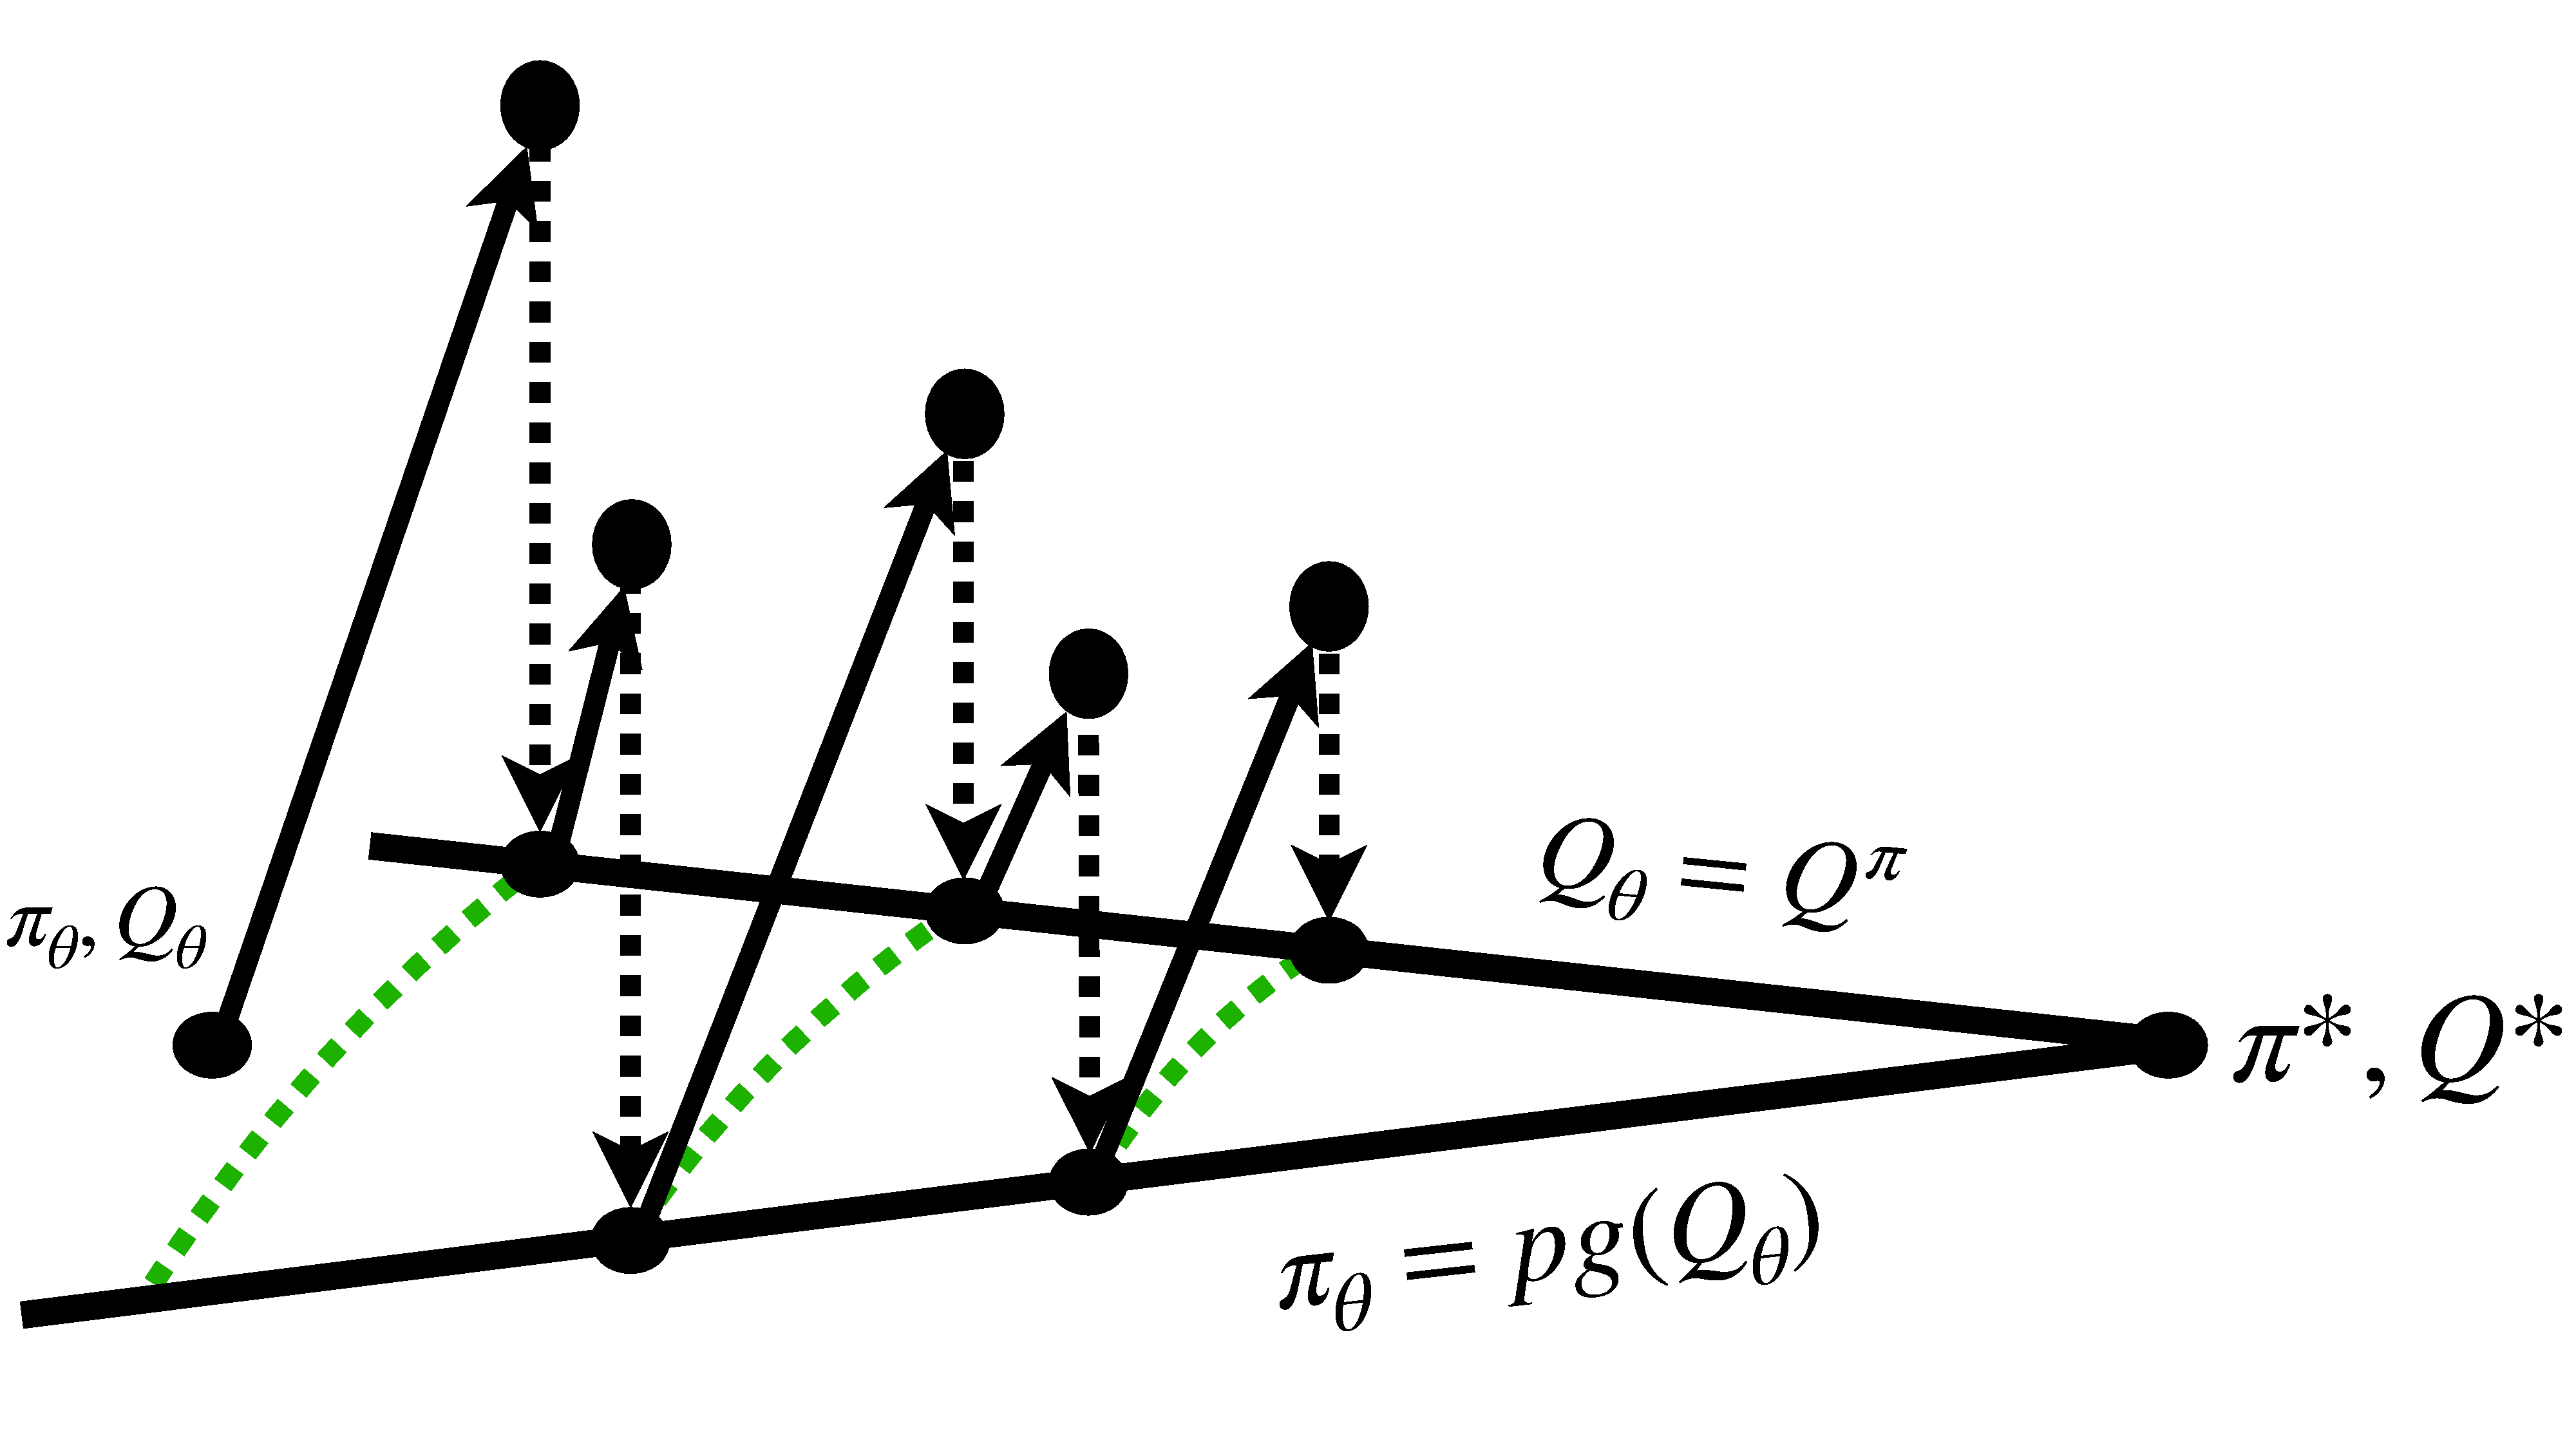
\includegraphics[width=0.4\textwidth,bb= 0 0 1800 1100]{body/figures/GPI2.pdf}
% \caption{
% GPI with function approximation.
% The black arrows represent the policy improvement and the policy evaluation. 
% The dotted arrows represent the projection into the approximated function space.
% The learning process is represented by the black arrows and dotted arrows, $ \textbf{I} \rightarrow \textbf{P}_\textbf{I} \rightarrow \textbf{E} \rightarrow \textbf{P}_\textbf{E} \rightarrow \cdots$.}
% \label{fig:gpi2}
% \end{figure}

Next, we assume the representation capacity of the approximation function is limited.
When the function approximation is involved, i.e. $Q^\pi$ is estimated by $Q_\theta$ and $\pi$ is approximated by $\pi_\theta$, from the view of operators ~\citep{op_reinforce}, each of \textbf{I} and \textbf{E} can be further decomposed into two operators, as shown in Figure \ref{fig:gpi2}.
One is to do the policy improvement and the policy evaluation, the other is to project into the restricted function space.
% We use $\textbf{P}_{*}$ to represent the projection into the approximated function space of $*$. 
When $\beta > 0$, GPI with function approximation would involve two projection operators in each iteration, which introduces inevitable approximation error.
When $\beta = 0$, if the function approximation error is not considered, we find that the gradient conflict between \textbf{I} and \textbf{E} would be totally eliminated.
If we consider the limitation of the approximation function, similar to the blue arrow in Figure \ref{fig:gpi}, one iteration (represented by two black arrows and two dotted arrows) can be united into one arrow and one dotted arrow (not shown in Figure \ref{fig:gpi2} but analogy to the blue arrow in Figure \ref{fig:gpi}), where the gradient conflict is eliminated and the two projection operators are reduced to one correspondingly.

As stated above, if $\beta = 0$ holds, we can expect that the gradient conflict between the policy improvement and the policy evaluation is eliminated and the function approximation error could be reduced. 
{\colorred However, $\beta$ is usually estimated by sampling with stochasticity. 
It's difficult to let $\beta = 0$ by optimizing $\theta$. 
Instead, we consider another notion $\chi$ by removing step sizes and taking expectation outside, where the angle of each state is fully controllable by $\theta$.
\begin{equation}
    \chi \overset{def}{=} \mathbb{E}_\pi [\cos <\nabla_\theta Q_\theta, \nabla_\theta \log \pi_\theta>].
\end{equation}
In fact, $\chi$ is highly correlated to compatible value function \citep{sutton1999policy},
and Theorem \ref{thm:connect_cond} shows that $\chi = 1$ is the necessary condition for the compatible condition $\nabla_\theta Q_\theta = \nabla_\theta \log \pi_\theta$, which is a weaker compatible condition.
More details about compatible value function are in Appendix \ref{app:comp_v}.
}

% Note that the importance of $\beta = 0$ has been considered by some earlier works, such as  
% the policy gradient theorem with function approximation \citep{sutton1999policy}. 
% % Considering the significance, 
% Further details on the theorem with notations could be found in Theorem \ref{thm:pg_fa} from Appendix \ref{app:mtv} .
\begin{figure}[t!]
	\centering
% 	\vskip 0.2in
	\begin{minipage}[c]{0.75\textwidth}
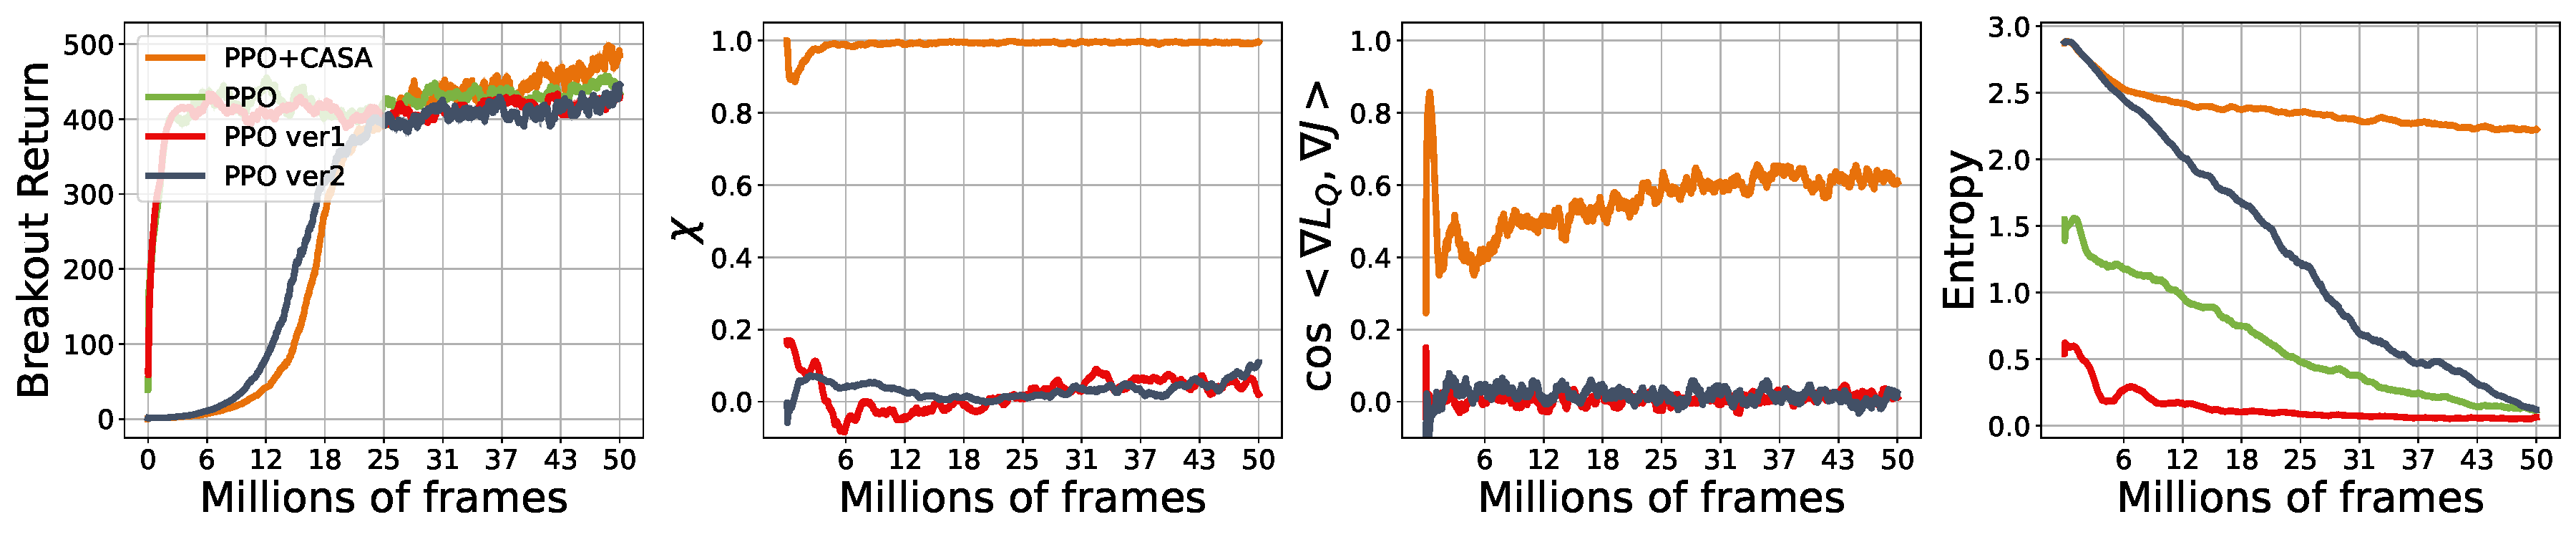
\includegraphics[width=\linewidth]{body/intro_fig/new_mtv_Breakout.pdf}
% 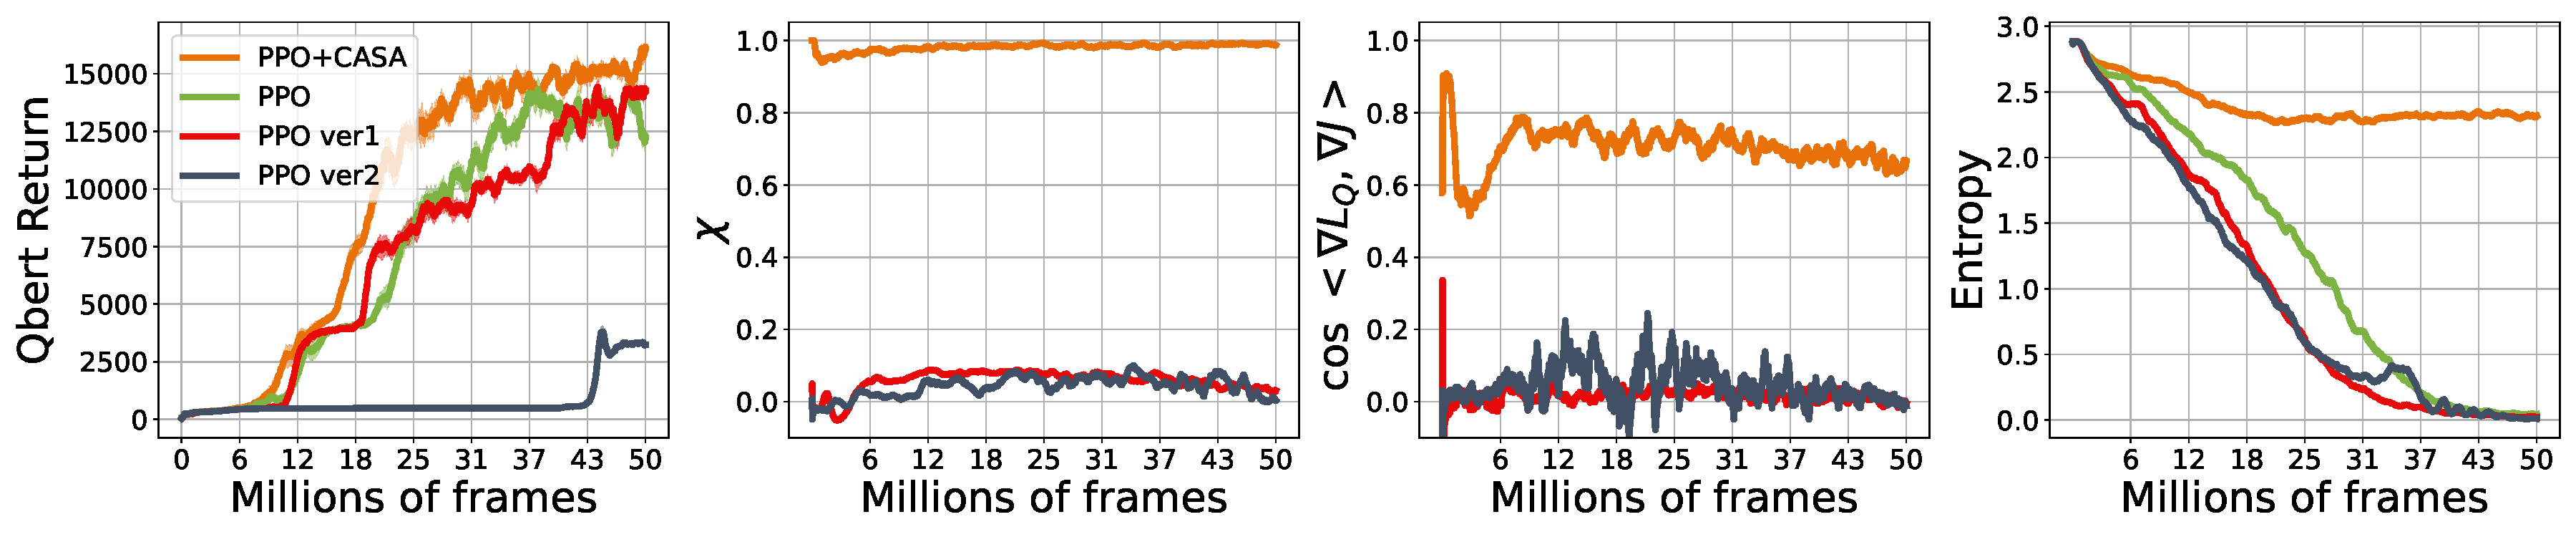
\includegraphics[width=\linewidth]{body/intro_fig/new_mtv_Qbert.pdf}
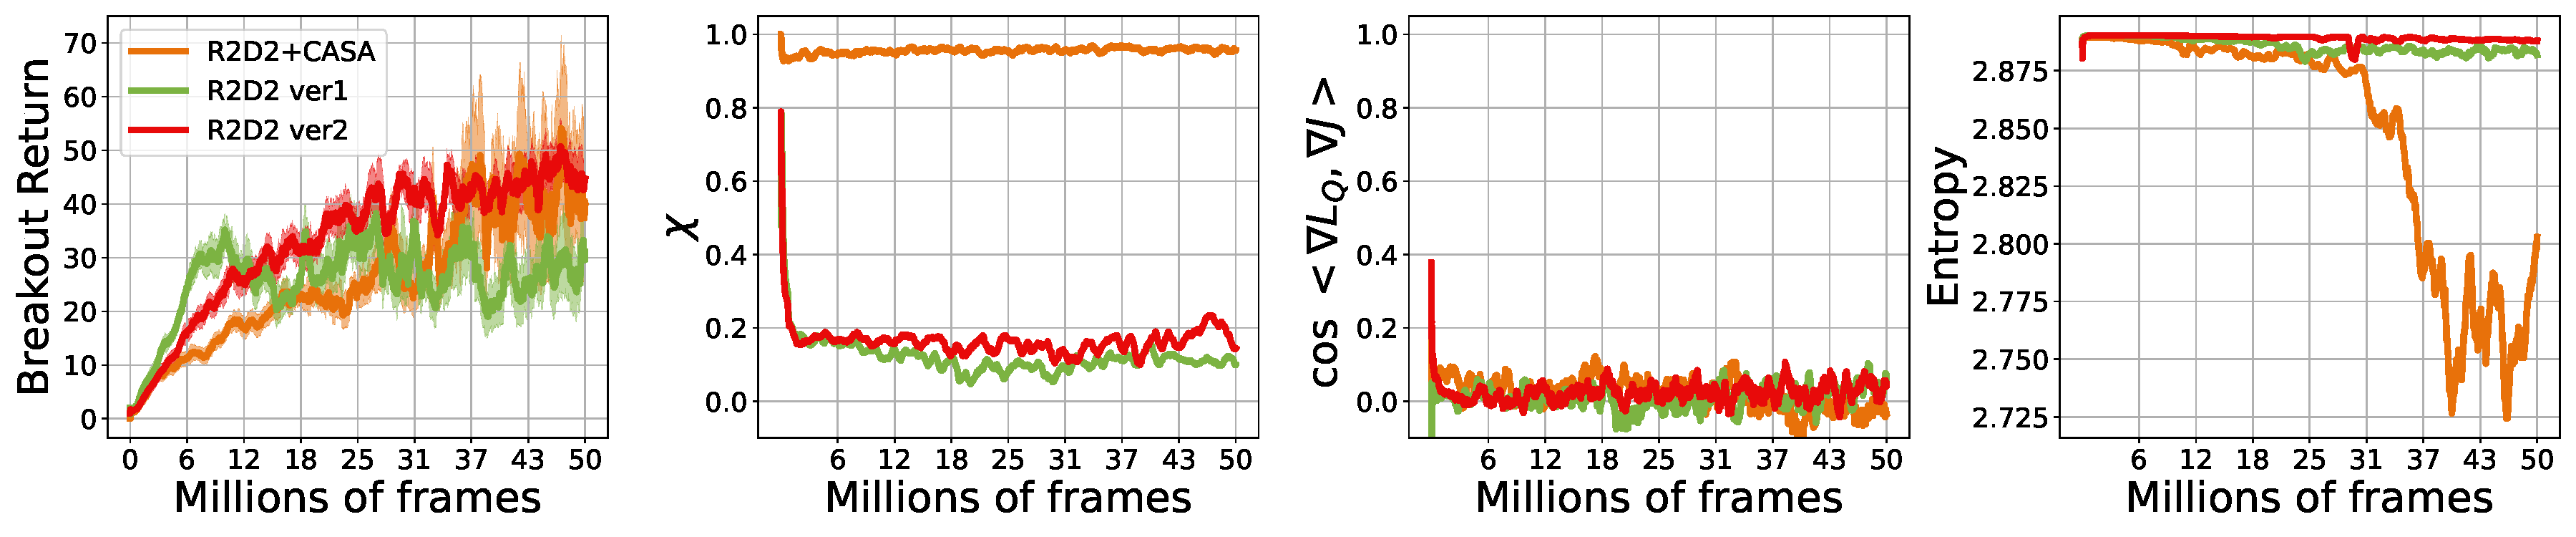
\includegraphics[width=\linewidth]{body/intro_fig/new_r2d2_mtv_Breakout.pdf}
% 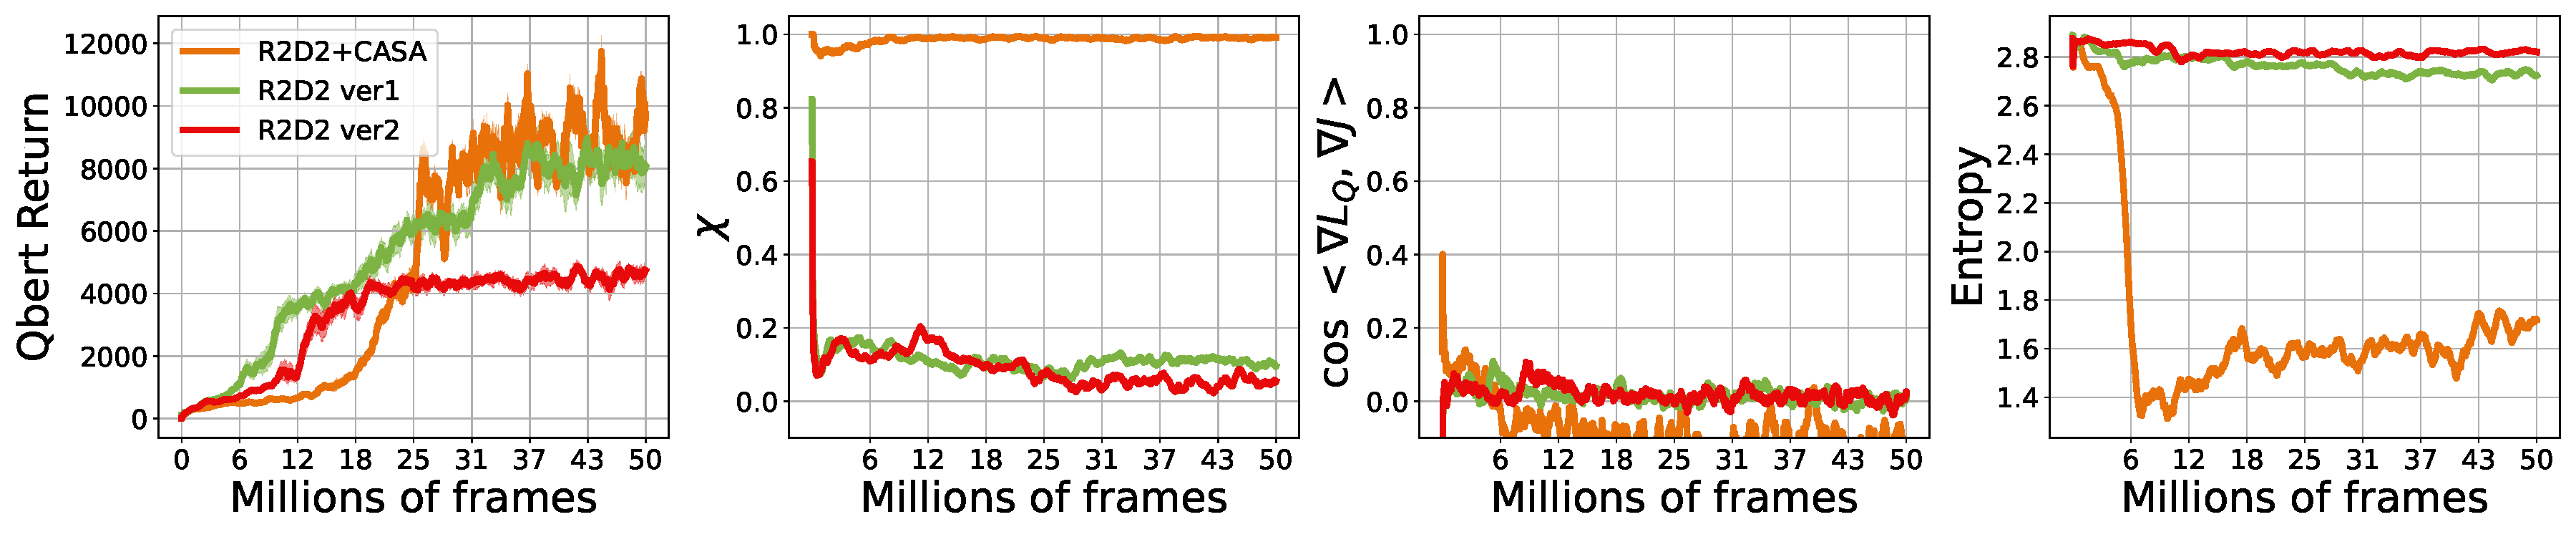
\includegraphics[width=\linewidth]{body/intro_fig/new_r2d2_mtv_Qbert.pdf}
  \end{minipage} \hfill
  \begin{minipage}[c]{0.23\textwidth}
    \caption{
    \small
    \emph{Return}, $\chi$, $\cos(\beta)$ and \emph{entropy}. PPO is adjusted with two additional versions to evaluate state-action values. R2D2 uses a surrogate policy to approximate policy gradient. Entropy of R2D2 is entropy of Boltzmann policy on state-action values. 
    %Angles between policy gradient and evaluating state values for PPO, and angles between evaluating state-action values and state values for R2D2 are both positive. 
    Details are in Appendix \ref{app:mtv}.}
    \label{fig:mtv}
    \end{minipage}
\end{figure}

To further understand the behavior of $\beta$ {\colorred and $\chi$}, we track $\cos(\beta)$ {\colorred and $\chi$} of two algorithms PPO and R2D2  as representatives for policy-based and value-based methods, respectively. We show an important fact in Figure \ref{fig:mtv} that {\colorred both $\chi$ and $\cos(\beta)$ are statistically positive for both original version and adjusted versions,
% This is reflected by the fact that cosines of angles between policy gradient and gradient of evaluating state values for PPO are always positive, and cosines of angles between gradients of evaluating state-action values and state values for R2D2 are always positive. 
which means that $\arccos(\chi)$ and $\beta$ are likely to be less then $\pi / 2$ with neural network approximated functions.}
% More details on this motivating experiment can be found in Appendix \ref{app:mtv}. 
% \jjf{need to polish the caption} 
% \changnan{make an example}
% Each value-based method and policy-based method has its own merits and shortcomings.
% This motivates us to find a trade-off between value-based methods and policy-based methods to inherit their merits and to mitigate their drawbacks.
The aforementioned conceptual and empirical findings  inspire us to raise the following question on GPI:
% Although MaxEnt suffers from some drawbacks, it's pretty close to unify value-based methods and policy-based methods. 
% One observation is that $\mathcal{J}_{soft}$ involves $\textbf{H}[\pi]$ into $\mathcal{J}$, which bridges the policy evaluation and the policy improvement.
% When we restrict the objective back to $\mathcal{J}$, it's reasonable to conjecture that the policy evaluation and the policy improvement should be different, i.e. 
% where $\nabla \mathcal{J} = \mathbb{E}_\pi [(G - V) \nabla \log \pi]$. 
% As $G-V$ and $G-Q$ represent the step size of the policy improvement direction $\nabla \log \pi$ and the policy evaluation direction $\nabla Q$ respectively, and $G-V \neq G-Q$, we won't expect the policy evaluation and the policy improvement to be equivalent, as long as we want to $maximize\ \mathcal{J}$.
% But inspired by the operator view ~\citep{op_reinforce}, we conjecture a \textit{weaker} consistent property that the policy improvement might be compatible with the policy evaluation: 
% under what condition, the policy improvement and the policy evaluation could share the same ascent direction in their gradients, i.e. $\nabla_\theta Q_\theta \propto \nabla_\theta \log \pi_\theta$?
{\colorred whether we can guarantee $\chi = 1$, so that $\cos(\beta)$ is also closer to $1$.}

% \begin{figure}[ht]
% \centering
% 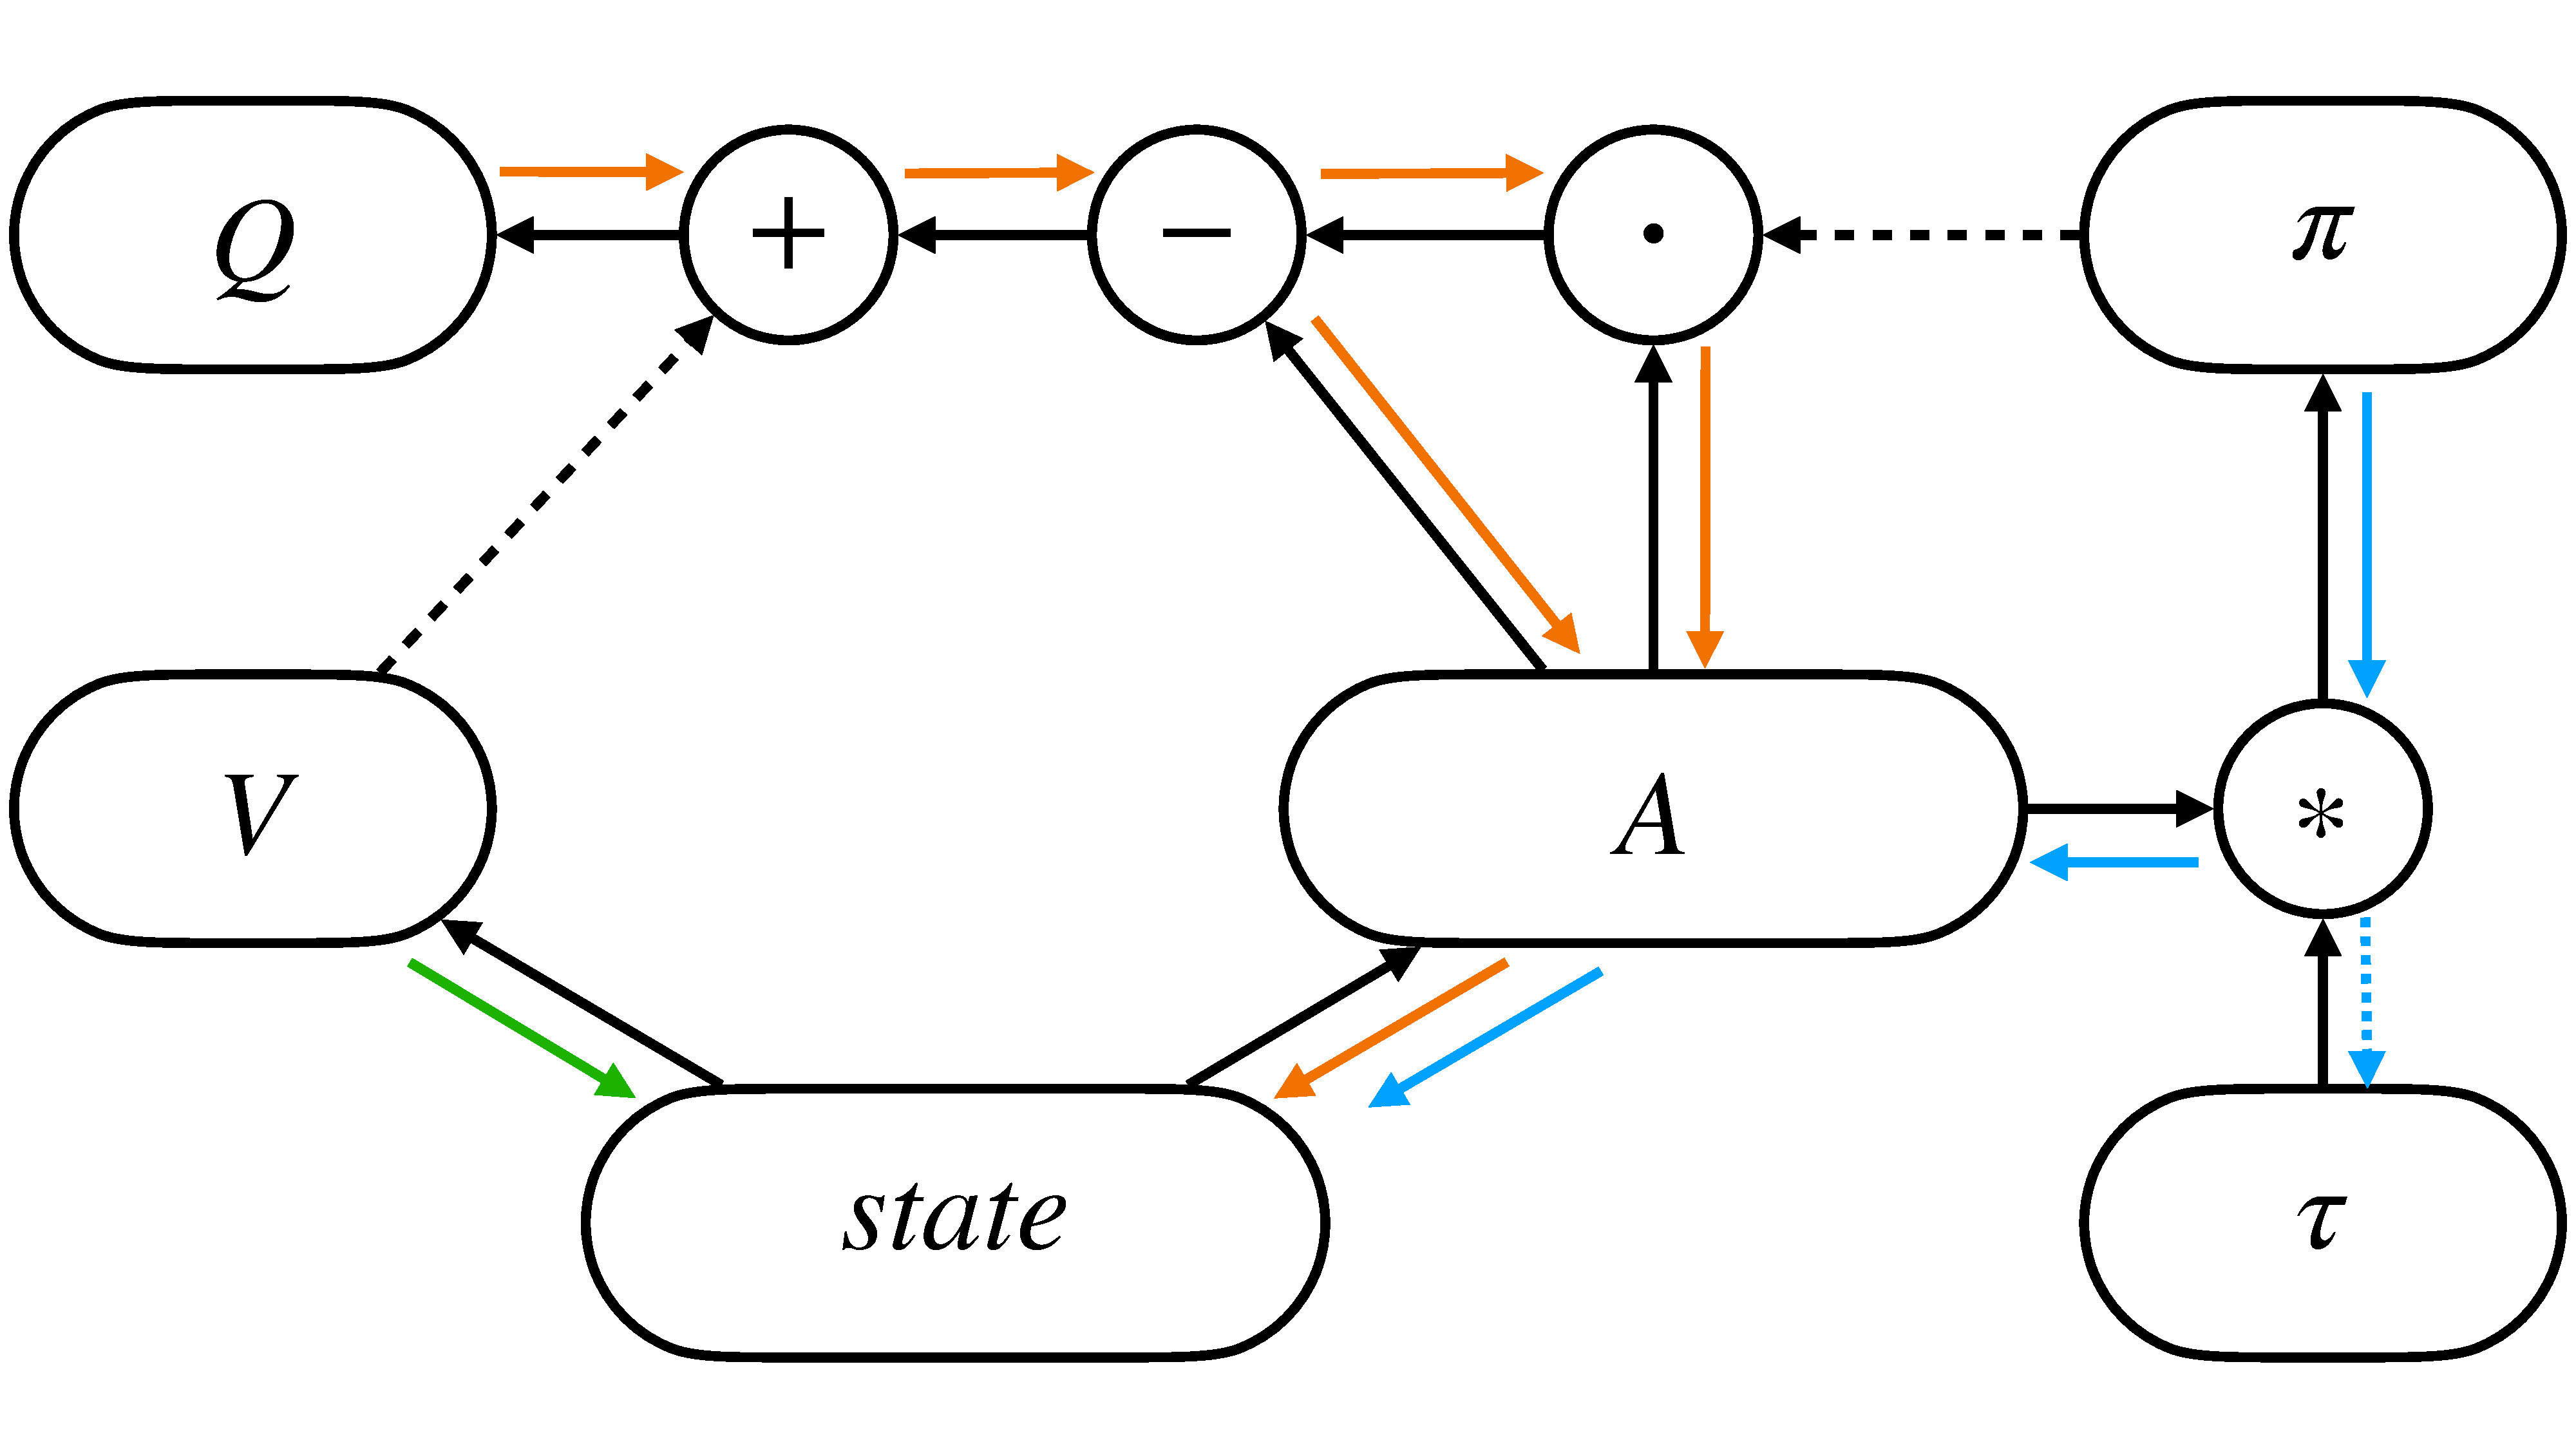
\includegraphics[height=4.5cm]{figure/CASA.pdf}
% \caption{
% \textbf{Black} lines represent the forward process.
% \textbf{Dotted} black lines represent the \textit{stop gradient} operator in the forward process. 
% \textbf{Colorful} lines represent backpropagation from different loss functions. 
% Specifically, \textbf{blue} lines represent $\mathbb{E}_\pi [(G-V)\nabla \log \pi]$, 
% \textbf{orange} lines represent $\mathbb{E}_\pi [(G-Q)\nabla Q]$,
% and \textbf{green} lines represent $\mathbb{E}_\pi [(G-V)\nabla V]$.}
% \label{fig:casa}
% \end{figure}



\subsection{Formulation}
\label{sec:formula}


% \changnan{one page deleted here.}
% We use $V_{\theta}$ to estimate $V^\pi$ and $A_{\theta}$ to estimate $A^\pi$.
% Let's start from the Boltzmann policy\footnote{The Boltzmann policy is a form of policy which is represented by a Boltzmann distribution and $softmax(\{v_i\}) = \{\exp(v_i) / \sum \exp(v_i)\}$.
% }, $\pi = softmax(A_\theta / \tau)$,
% where $A_\theta:\mathcal{S} \rightarrow \mathbb{R}^{|\mathcal{A}|}$ is a parameterized function. %$A_\theta = Q_\theta - V_\theta$.
% % which is
% % $$
% % \pi = \exp(A / \tau) / Z,\ Z = \int_\mathcal{A} \exp(A / \tau).
% % $$
% % Notice that $\pi$ is a function of $A_\theta$ and $A_\theta$ is a parameterized function of $(s, a)$.
% We want to find a function $Q$ satisfying $\nabla_\theta Q \propto \nabla_\theta \log \pi$ for $\forall\ \theta$.

% In order to build the connection between $Q$ and $\log \pi$, we assume that $Q$ is a function of two parts. The first part is $A_\theta$ which can complete decide the policy $\pi$ and the other is $V_\theta:\mathcal{S}\rightarrow \mathbb{R}$ which is a function only depend on states. i.e. $ Q_\theta = f(A_\theta, V_\theta)$. 
% % We will show that the assumption is sufficient. 
% % 
% \begin{lemma}
% Let 
% $g \in \textbf{C}^{1}(\mathbb{R}^{n}): \mathbb{R}^{n} \to \mathbb{R}^{n}, \ f \in \textbf{C}^{1}(\mathbb{R}^{n+k}): \mathbb{R}^{n+k} \to \mathbb{R}^{n}.
% $
% If
% $
% \nabla_x g(x) = \nabla_x f(x, y)$, for $\forall x\in \mathbb{R}^{n}, y\in \mathbb{R}^k,
% $
% then $\exists$ $c \in \textbf{C}^{1}(\mathbb{R}^{k}): \mathbb{R}^{k} \to \mathbb{R}^{n}$, s.t. $f(x, y) = g(x) + c(y)$.
% \label{lemma:func_sep}
% \end{lemma}
% \begin{proof}
% See Appendix \ref{app:proof}, Lemma \ref{lemma_app:func_sep}.
% \end{proof}
% Regarding $x = A_\theta$ to be any vector in $\mathbb{R}^{|\mathcal{A}|}$, $y = V_\theta$ to be any vector in $\mathbb{R}^1$, $g = \pi(\cdot|s) = \log softmax(A_\theta / \tau)$ to be a function of $A_\theta$ and $f = Q = f(A_\theta, V_\theta)$ to be a function of $A_\theta$ and $V_\theta$ in Lemma \ref{lemma:func_sep}, let $\theta = A_\theta$ in $\nabla_\theta Q \propto \nabla_\theta \log \pi$, we know 
% $$
% \begin{aligned}
%         Q &= f(A_\theta, V_\theta) 
% % = \log \pi + c (V_\theta) 
% = \log softmax(A_\theta / \tau) + c (V_\theta) \\
% &\triangleq f_1 (A_\theta) + c (V_\theta).
% \end{aligned}
% $$

% According to the Bellman equation $\mathbb{E}_\pi [Q] = V_\theta$, we have
% $$
% \mathbb{E}_\pi [f_1 (A_\theta)] = \mathbb{E}_\pi [V_\theta - c (V_\theta)] = V_\theta - c (V_\theta).
% $$
% Since $\mathbb{E}_\pi [f_1 (A_\theta)]$ is not a function of $V_\theta$, regarding $V_\theta$ as a vector in $\mathbb{R}^1$ and taking $\partial / \partial V_\theta$ on both sides, we have that $V_\theta - c (V_\theta)$ is a constant function. 
% Without loss of generality, assume $V_\theta - c (V_\theta) = 0$, as we can minus this constant on both sides.

% Now we know $Q = f_1(A_\theta) + V_\theta$.

% Since we will not change $V_\theta$ when doing the policy improvement, we have $\partial \log \pi / \partial V_\theta = 0$.
% Noting that $\nabla_\theta Q \propto \nabla_\theta \log \pi \Rightarrow \partial_\theta Q / \partial_\theta V_\theta \propto \partial_\theta \log \pi / \partial_\theta V_\theta = 0$, we stop the gradient of $V_\theta$ in $Q = f_1(A_\theta) + V_\theta$. 
% Hence, we solve for $f_1$ s.t. $\nabla_\theta f_1(A_\theta) \propto \nabla_\theta \log \pi$.

% \begin{lemma}
% (i) Define $\pi = softmax(A / \tau)$, then $\nabla \log \pi = (\textbf{1} - \pi) \frac{\nabla A}{\tau}$.
% (ii) Denote $sg$ to be stop gradient and define $\Bar{A} = A - \mathbb{E}_\pi [A]$, $Q = \Bar{A} + sg(V)$, then $\nabla Q = (\textbf{1} - \pi) \nabla A$.
% \label{lemma:vannila_grad}
% \end{lemma}
% \begin{proof}
% See Appendix \ref{app:proof}, Lemma \ref{lemma_app:vannila_grad}.
% \end{proof}
% Let $A = A_\theta$ in Lemma \ref{lemma:vannila_grad} (i), we have 
% $$
% \nabla_\theta \log \pi = \frac{1}{\tau} (\textbf{1} - \pi) \nabla_\theta A_\theta.
% $$
% Notice that $\nabla_\theta f_1(A_\theta)$ is the gradient ascent direction of the policy evaluation and $\nabla_\theta \log \pi$ is the gradient ascent direction of the policy improvement.
% Since $\pi$ is a constant when doing the policy evaluation,
% when solving for $\nabla_\theta f_1(A_\theta) \propto \nabla_\theta \log \pi$, we regard $\pi$ as a constant and integrate $(\textbf{1} - \pi) \nabla_\theta A_\theta$, then
% $$
% f_1(A_\theta) \propto (\textbf{1} - \pi) A_\theta + constant.
% $$
% Again, since $\mathbb{E}_\pi [Q] = V_\theta \Rightarrow \mathbb{E}_\pi [f_1(A_\theta)] = 0$, we know 
% $$
% Q = (\textbf{1} - \pi) A_\theta + V_\theta = A_\theta - \mathbb{E}_\pi [A_\theta] + V_\theta.
% $$

% Reformatting the above derivation, we have the forward process of CASA.
% \changnan{The above calculations are not formal. Will be moved to appendix as an intuitive induction.}



Denote $\tau \in \mathbb{R}_+$ to be a positive temperature and $sg$ to be a $stop\ gradient$ operator. 
CASA can estimate $V_\theta$ and $A_\theta$ by any function parameterized by $\theta$, where $\pi_\theta$ and $Q_\theta$ are derived as follows:
\begin{equation}
\label{eq:casa}
\left\{
    \begin{aligned}
        &\pi_\theta(\cdot|s) = \text{softmax}(A_\theta(s, \cdot) /
        \tau), \\
        % &\Bar{A}_\theta(s, a) &= A_\theta(s, a) - \mathbb{E}_{\pi}[A_\theta] \\
        &\Bar{A}_\theta(s, a) = A_\theta(s, a) - \sum_{a'} sg(\pi_\theta(a'|s)) A_\theta(s, a'), \\
        % \footnotemark
        &Q_\theta(s, a) = \Bar{A}_\theta(s, a) + sg(V_\theta(s)).
    \end{aligned}
\right. 
% \addtocounter{footnote}{-1}
% \footnotetext{$/$ represents element-wise multiplication.}
% \stepcounter{footnote}
% \footnotetext{$\mathbb{E}_{\pi}[A_\theta] = sg(\pi) \cdot A_\theta$, where $\cdot$ represents inner product.}
\end{equation}

% We provide a summary of the structure as shown in Appendix Figure \ref{fig:casa}.
Note that there exist two $sg$ operators in \eqref{eq:casa}.
The first $sg$ operator is used for computing advantage as $\Bar{A}_\theta = A_\theta - \mathbb{E}_\pi [A_\theta] = A_\theta - sg(\pi_\theta) \cdot A_\theta$,
% This $sg$ operator guarantees the path consistency between the policy improvement and the policy evaluation, 
% shown later in \eqref{eq:vannila_grad}.
where the $sg$ operator here guarantees the gradients between policy improvement and policy evaluation are parallel, which we elaborate later.
Intuitively, this $sg$ operator also means that we keep $\pi_\theta$ unchanged when evaluating the policy $\pi_\theta$.
The second $sg$ operator exists in $Q_\theta = \Bar{A}_\theta + sg(V_\theta)$.
% This $sg$ operator is crucial in the convergence proof of Theorem \ref{thm:dr}.
As ~\citep{simsiam} regards $sg$ in siamese representation learning as a case of EM-algorithm ~\citep{em}, a similar interpretation exists here.
$Q_\theta = \Bar{A}_\theta + sg(V_\theta)$ decomposes the estimation of $Q_\theta$ into a two stage problem, where the first is to estimate the advantage of each action without changing the expectation, the second is to estimate the expectation.
% More details are concluded in the proof of Theorem \ref{thm:dr}.
% \ifnum2=0\mytestvar

The \eqref{eq:casa} includes a straightforward refinement of dueling-DQN.
% We know dueling-DQN estimates $Q_\theta$ by $Q_\theta =  A_\theta + V_\theta$, which corresponds to:
% $$
% Q^{\pi} (s_t, a_t) = \mathbb{E}_p [r_t + \gamma 
%     V^{\pi}(s_{t+1}) - V^{\pi}(s_t)] + V^{\pi}(s_t).
% $$
% Since $\mathbb{E}_{\pi} [ \mathbb{E}_p [r_t + \gamma V^{\pi}(s_{t+1}) - V^{\pi}(s_t)]] = 0$, we have
% $$
% \begin{aligned}
%     Q^{\pi} (s_t, a_t) 
%     =  \mathbb{E}_p [r_t + \gamma V^{\pi}(s_{t+1}) - V^{\pi}(s_t)]
%      - \mathbb{E}_\pi [ \mathbb{E}_p [r_t + \gamma V^{\pi}(s_{t+1}) - V^{\pi}(s_t)]] + V^{\pi}(s_t),
% \end{aligned}
% $$
% which is $Q_\theta = A_\theta - \mathbb{E}_\pi [A_\theta] + V_\theta$.
{\colorred We know dueling-DQN estimates $Q^\pi$ by $Q_\theta =  A_\theta + V_\theta$, but it cannot guarantee $\mathbb{E}_\pi[A_\theta] = 0$ i.e. $\mathbb{E}_\pi [Q_\theta] = V_\theta$ due to the function approximation error. 
But if we estimate $Q_\pi$ by $Q_\theta =  A_\theta - \mathbb{E}_\pi[A_\theta] + V_\theta$, it satisfies the necessary condition $\mathbb{E}_\pi [Q_\theta] = V_\theta$ without loss of generality.}

\subsection{Path Consistency Between Policy Evaluation and Policy Improvement}
\label{sec:equiv}

% In section \ref{sec:dr}, policy evaluation and policy improvement are actually separated, entangled structure of $\pi$ and $Q$ defined in \eqref{eq:casa} is not involved.
For brevity, we omit $\theta$ and $V, Q, A, \pi$ are all approximated functions.
% Now we discuss how the policy evaluation and the policy improvement affect each other.
Denote the estimations of $V$ and $Q$ as $V^{\Tilde{\pi}}$ and $Q^{\Tilde{\pi}}$ respectively. For instance, one choice is to calculate $V^{\Tilde{\pi}}$ and $Q^{\Tilde{\pi}}$ by V-Trace ~\citep{impala} and ReTrace ~\citep{retrace} respectively.

At training time, the policy evaluation is achieved by updating $\theta$ to minimize,
$$
\begin{aligned}
    L_V(\theta) = \mathbb{E}_\pi [ (V^{\Tilde{\pi}} - V)^2 ], \ 
    L_Q(\theta) = \mathbb{E}_\pi [ (Q^{\Tilde{\pi}} - Q)^2 ],
\end{aligned}
$$ 
which gives the ascent direction of $\theta$ by:
\begin{equation}
\label{eq:grad_qv}
    \begin{aligned}
        \nabla_\theta L_V(\theta)
        = \mathbb{E}_\pi \left[ (V^{\Tilde{\pi}} - V) \nabla_\theta V \right], \ 
        \nabla_\theta L_Q(\theta)
        = \mathbb{E}_\pi \left[ (Q^{\Tilde{\pi}} - Q) \nabla_\theta Q \right].
    \end{aligned}
\end{equation}
And we make the policy improvement by policy gradient, which gives the ascent direction of $\theta$ by: 
\begin{equation}
\label{eq:grad_pi}
\begin{aligned}
    \nabla_\theta \mathcal{J}(\tau, \theta) = \mathbb{E}_\pi \left[\tau (Q^{\Tilde{\pi}}  - V ) \nabla_\theta \log \pi \right],
\end{aligned}
\end{equation}
where $\mathcal{J} (\tau, \theta) = \tau \mathbb{E}_\pi [\sum \gamma^t r_t]$.
It takes an additional $\tau$, which frees the scale of gradient from $\tau$.

The final gradient ascent direction of $\theta$ is given by:
\begin{equation}
    \label{eq:grad_all}
    \alpha_1 \nabla_\theta L_V + \alpha_2 \nabla_\theta L_Q + \alpha_3 \nabla_\theta \mathcal{J}.
\end{equation}

With $(V, Q, \pi)$ defined in \eqref{eq:casa}, 
by Lemma \ref{lemma_app:vannila_grad}, we have, 
\begin{equation}
    \label{eq:vannila_grad}
\nabla_\theta Q =  (\textbf{1} - \pi) \nabla_\theta A = \tau \nabla_\theta \log \pi .
\end{equation}
For brevity, denote the shared gradient path as
$\textbf{g} = (\textbf{1} - \pi) \nabla_\theta A.$

Plugging \eqref{eq:vannila_grad} into \eqref{eq:grad_qv} \eqref{eq:grad_pi}, we have,
\begin{equation}
\label{eq:grad_qv_simple}
\begin{aligned}
        \nabla_\theta L_Q = \mathbb{E}_\pi \left[ (Q^{\Tilde{\pi}} - Q) \textbf{g} \right], 
\nabla_\theta \mathcal{J} = \mathbb{E}_\pi \left[ (Q^{\Tilde{\pi}} - V) \textbf{g} \right].
% \footnotemark
\end{aligned}
% \footnotetext{$Q_t^{\Tilde{\pi}} = Q_{DR}^{\Tilde{\pi}} (s_t, a_t)$, $Q_t = Q(s_t, a_t)$, $V_t = V(s_t)$.}
\end{equation}
% \changnan{one paragraph deleted.}
% Recalling Theorem \ref{thm:dr}, when the importance sampling ratio $\Bar{\rho} = +\infty$ and we ignore the bias introduced by the function approximation error, we know $Q_t^{\Tilde{\pi}}$ is an unbiased estimation of $\mathbb{E}_\pi [G_t | s_t, a_t]$.
% Based on this observation, $\nabla_\theta L_Q$ is a typical policy evaluation that $Q$ converges to $\mathbb{E}_\pi [\sum \gamma^k r_{k} | s, a]$, 
% and $\nabla_\theta \mathcal{J}$ is a typical policy improvement that maximizes $\mathbb{E}_\pi [\sum \gamma^k r_k]$. 
% $\nabla_\theta L_Q$ and $\nabla_\theta \mathcal{J}$ are expected to be different, as $Q$ and $V$ are updated by the Bellman equation,
% rather than the \textit{soft} Bellman equation.
{\colorred By \eqref{eq:grad_qv_simple}, $\nabla_\theta L_Q$ and $\nabla_\theta \mathcal{J}$ walk along the same vector direction of gradient path $\textbf{g}$ for each state.}
% By \eqref{eq:grad_qv_simple}, the directions of the gradients $\textbf{g}$ are in common. 
% We call it a path. 
% The \eqref{eq:grad_qv_simple} shows that $\nabla_\theta L_Q$ and $\nabla_\theta \mathcal{J}$ walk along the same path $\textbf{g}$. 
% The difference is that $\nabla_\theta L_Q$ walks with step size $Q^{\Tilde{\pi}} - Q$, but $\nabla_\theta \mathcal{J}$ walks with step size $Q^{\Tilde{\pi}} - V$. 
{\colorred By \eqref{eq:vannila_grad}, this is exactly the case $\chi = 1$.}
Since all parameters to estimate $Q$ and $\pi$ are shared except for $\tau$, we call it \textbf{C}ritic \textbf{AS} an \textbf{A}ctor.

If we make a subtraction between $\nabla_\theta L_Q$ and $\nabla_\theta \mathcal{J}$, we have,
\begin{equation}
\label{eq:grad_relation}
    \nabla_\theta \mathcal{J} = \nabla_\theta L_Q + \mathbb{E}_\pi \left[(Q - V) \textbf{g} \right].
\end{equation}
% We know $\mathbb{E}_\pi \left[ (Q_t - V_t) \textbf{g} \right]$ is also a policy gradient with function approximated $Q_t$. 
We know $\mathbb{E}_\pi \left[ (Q - V) \textbf{g} \right]$ is a self-bootstrapped policy gradient with function approximated $Q$.
% \changnan{one paragraph deleted.}
% If we regard $Q_t^{\Tilde{\pi}}$ as a \textit{better} estimation of $Q_t$, \eqref{eq:grad_relation} says that the policy evaluation equals to the policy improvement minus a \textit{worse} policy improvement, which is to retain the policy evaluation by pulling back from the policy improvement. 
% As for how \textit{worse} it is, it depends on how far $Q_t$ is from $Q_t^{\Tilde{\pi}}$. 
% Recalling \eqref{eq:grad_qv_simple} and $\textbf{g} = \tau \nabla_\theta \log \pi$, we observe that if $Q_t$ underestimates $Q_t^{\Tilde{\pi}}$, $\nabla_\theta L_Q$ promotes $\pi(a_t|s_t)$ by $Q_t^{\Tilde{\pi}} - Q_t$, otherwise $\nabla_\theta L_Q$ diminishes $\pi(a_t|s_t)$ by $Q_t^{\Tilde{\pi}} - Q_t$. 
% So except for the policy evaluation, $\nabla_\theta L_Q$ does do policy improvement along the same path as $\nabla_\theta \mathcal{J}$, but only to compensate the estimation error of $Q_t$.
% If we regard $Q^{\Tilde{\pi}}$ as a \textit{better} estimation of the ground truth state-action values than $Q$, the \eqref{eq:grad_relation} says that the policy improvement equals to the policy evaluation plus a \textit{worse} policy improvement, where the \textit{worse} policy improvement entirely depends on the evaluated values. 
Recalling the fact that the value-based methods improves the policy by greedily selecting actions according to $Q$, if we apply $\nabla_\theta \mathcal{J}$ on $\theta$, it additionally utilizes $Q$ to do policy improvement. 
This is a more greedy usage of $Q$ to improve policy than its usual usage. 

% \changnan{one lemma deleted.}
% \begin{lemma}
% Define $\Bar{A}= A - \mathbb{E}_\pi[A]$, $Q = \Bar{A} + sg(V), \pi = softmax(A / \tau)$, then 
% $
% \mathbb{E}_\pi \left[ (Q - V) \nabla \log \pi \right]
% = - \tau \nabla \textbf{H}[\pi].
% $
% \label{lemma:eqiv_pg_ent}
% \end{lemma}
% \begin{proof}
% See Appendix \ref{app:proof}, Lemma \ref{lemma_app:eqiv_pg_ent}.
% \end{proof}

% Now we know $\nabla_\theta L_Q$ is not only a policy evaluation but is also equivalent to a compensational policy improvement. 
If we exploit the structural information as $(V, Q, \pi)$ defined by \eqref{eq:casa}, by Lemma \ref{lemma_app:eqiv_pg_ent},
$$
\mathbb{E}_\pi \left[(Q - V) \textbf{g} \right] 
= \tau \mathbb{E}_\pi \left[(Q - V) \nabla_\theta \log \pi \right]
= - \tau^2 \nabla_\theta \textbf{H}[\pi],
$$
then we have,
\begin{equation}
\label{eq:ent_reg}
    \nabla_\theta L_Q 
    = \nabla_\theta \mathcal{J} + \tau^2 \nabla_\theta \textbf{H}[\pi].
\end{equation}

The \eqref{eq:ent_reg} shows $\nabla_\theta L_Q$ is a policy gradient with an entropy regularization.
If we apply $\nabla_\theta L_Q$ on $\theta$ for policy-based methods, an entropy regularization works implicitly by $\alpha_2 \nabla_\theta L_Q$ in \eqref{eq:grad_all}, which prevents the policy collapse to a sub-optimal solution. 
% An intuitive explanation is that, as $Q$ and $\pi$ share $A$, but the range of $Q$ is dominated by MDP, so $Q$ regularizes $A$ to prevent $\pi$ from collapse to sub-optimal solutions.

\subsection{DR-Trace and Off-Policy Training}
\label{sec:dr}

% In the previous section, we introduce how we estimate $(V, Q, \pi)$. 
% For brevity, we omit $\theta$ and $V, Q, A, \pi$ are all approximated functions.
% In this section, we introduce how we learn $(V, Q, \pi)$.

% \changnan{one page moved to appendix.}

\begin{table}[ht!]
 \vskip -0.05in
    \centering
    \vspace{0.1cm}
    \scalebox{0.82}{
    \begin{tabular}{c|c|c}
    \toprule
    
     & \text{{\color{blue}DR-Trace}} & \text{{\color{orange}V-Trace} / {\color{green}ReTrace}} \\
     \midrule
      & $\delta^{{\color{blue}DR}}_t {=} r_t + \gamma {\color{blue}V}(s_{t+1}) - {\color{blue}Q}(s_t, a_t)$ & $\delta^{{\color{orange} V}/{\color{green}Q}}_t {=} r_t + \gamma {\color{orange} V}(s_{t+1})/{\color{green}Q}(s_{t+1},a_{t+1}) - {\color{orange} V}(s_t)/{\color{green}Q}(s_t,a_t)$ \\
    \midrule
    $V^{\Tilde{\pi}}$ & $\mathbb{E}_{\mu} [V_t + \sum_{k \geq 0} \gamma^k c_{[t:t+k-1]} \rho_{t+k}  {\color{blue}\delta^{DR}_{t+k}}]$ & $\mathbb{E}_{\mu} [V_t + \sum_{k \geq 0} \gamma^k c_{[t:t+k-1]} \rho_{t+k}  {\color{orange}\delta^{V}_{t+k}} ]$ \\
    \midrule
    $Q^{\Tilde{\pi}}$  & $\mathbb{E}_{\mu}   [Q_t + \sum_{k \geq 0} \gamma^k {\color{blue}c_{[t+1:t+k-1]} ( 1_{\{k=0\}} + 1_{\{k > 0\}} \rho_{t+k}) \delta^{DR}_{t+k}} ]$ & $\mathbb{E}_{\mu}   [Q_t + \sum_{k \geq 0} \gamma^k {\color{green}c_{[t+1:t+k]} \delta^{Q}_{t+k}} ]$  \\ 
    \midrule
    $\nabla \mathcal{J}$ & $\mathbb{E}_{\mu} [\rho_t({\color{blue}Q_t^{\Tilde{\pi}}} - V_t)\nabla \log \pi]$ &  $\mathbb{E}_{\mu} [\rho_t({\color{orange}r_t + V_{t+1}^{\Tilde{\pi}}} - V_t)\nabla \log \pi]$ \\
    \bottomrule 
    \end{tabular}
    }
    \caption{Comparison between DR-Trace and V-Trace/ReTrace.}
    \label{tab:drtrace}
 \vskip -0.05in
\end{table}


{\colorred To enable off-policy training with behavior policy $\mu$}, one choice is to estimate $V^{\Tilde{\pi}}$ and $Q^{\Tilde{\pi}}$ in \eqref{eq:grad_qv} and \eqref{eq:grad_pi} by V-Trace and ReTrace. 
As CASA estimates $(V, Q, \pi)$, applying Doubly Robust ~\citep{dr} is feasible and suitable.
We propose DR-Trace and find the convergence rate and the fixed point of DR-Trace are the same as V-Trace's according to its convergence proof. 
For completeness, we provide DR-Trace and its comparison with V-Trace/ReTrace in Table \ref{tab:drtrace}. 
% Notations follow that of ~\citep{impala}'s, except for 
% $\Tilde{\rho}_{t, k} =  1_{\{k=0\}} + 1_{\{k > 0\}} \rho_{t+k}$, 
% $\delta^{DR}_t {=} r_t + \gamma V(s_{t+1}) - Q(s_t, a_t)$,
% $\delta^{V}_t {=} r_t + \gamma V(s_{t+1}) - V(s_t)$ and 
% $\delta^{Q}_t {=} r_t + \gamma Q(s_{t+1}, a_{t+1}) - Q(s_t, a_t)$.
More details are in Appendix \ref{app:drtrace}.

